\chapter{Model architecture and processes}
\label{ch:design}

In this chapter, both the architecture and the training and inference mechanisms of a concrete system are described. We begin introducing the overall architecture of the system, followed by specific sections devoted to the different parts of the system: encoder, decoder and attention mechanism. Finally, we describe the methods used to train and evaluate the system.

\section{Overview of the model architecture}

As we have discussed in previous section \cref{sec:scope}, we have decided to develop an end-to-end deep learning solution to the image captioning problem based on an \textbf{encoder-decoder architecture} with an \textbf{attention mechanism}. This is so far the most common architecture used by state of the art systems, as we have seen in our review of the field (\cref{ch:state_of_the_art}.) More specifically, our system will consist of the following components:

\begin{itemize}
    \item Encoder made of a Convolutional Neural Network (CNN)
    \item Decoder made of a Recurrent Neural Network (RNN)
    \item Soft Attention mechanism
\end{itemize}

\begin{figure}[hpt]
	\centering
	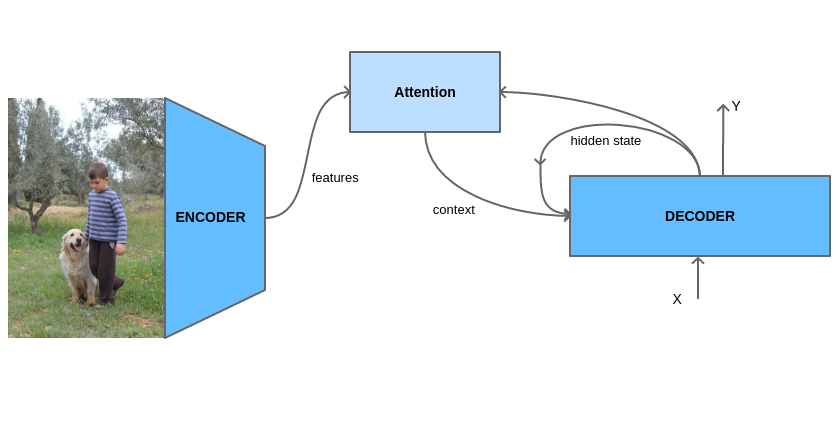
\includegraphics[scale=0.5]{images/ch4/overview.png}
	\caption{Overview of the model architecture: encoder, decoder and attention mechanism}
	\label{fig:overview}
\end{figure}

The general architecture of the system is depicted in \cref{fig:overall-architecture}. To the left of the figure, there is the encoder, which takes an image as input and extracts a feature map. To the right, the decoder has to produce a caption for the input image, using information from its input, its hidden state, as well as the context information received from the attention mechanism. The attention mechanism lies in between the encoder and the decoder. It is responsible of deciding on which parts of the image (on which features) to focus at each time step while. The attention mechanism take the image features and the hidden state of the decoder as inputs, and generates a context vector, which consists of the features weighted according to some learned weights, which represent the relevance given to each feature at a given moment.

Whilst the encoder generates the features in a single forward step, the decoder has to generate a caption word by word, one word at a time. To generate the next word it uses the information from past states, the current input (the last generated word), and the context information. The process of generating a caption as well as the training procedure will be describe later in this chapter.

A more detailed view of the architecture is provided in \cref{fig:overall-architecture}, showing the main layers used in the different components of the system. 
\begin{itemize}
    \item The encoder consists of a CNN module pretrained on the ImageNet dataset. We take the output from the last convolutional layer, and pass it through a dense, fully connected layer to flatten it before passing it to the attention module. 
    \item The decoder consists of an embedding layer that converts input tokens into embedding vectors, a recurrent layer, which may be made of either GRU or LSTM units, and two stacked fully connected layer that produce the final output. The input is a concatenation of the external input and the context vector from the attention mechanism.
    \item The attention mechanism actually consists of two fully connected layers, although they are not showed in the picture. It takes the flattenned features from the encoder as input, the hidden states from the decoder, computes attention weights and produces a context vector as output.
\end{itemize}


\begin{figure}[hpt]
	\centering
	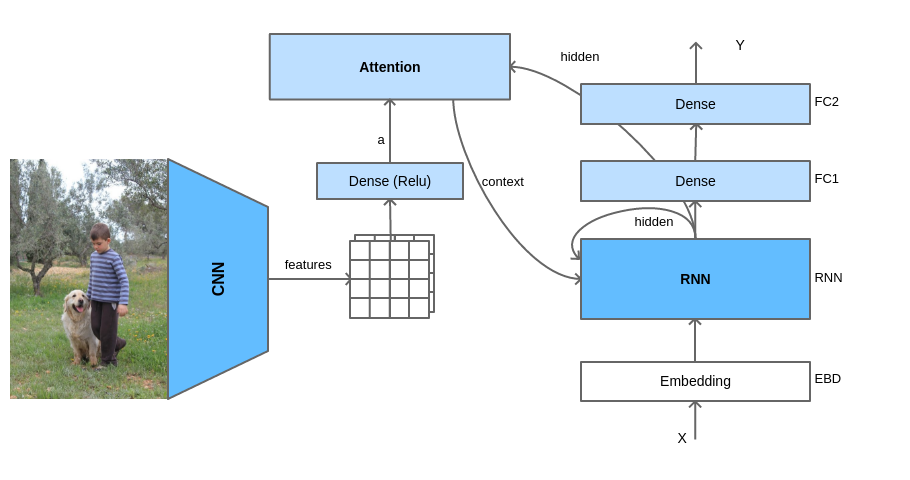
\includegraphics[scale=0.5]{images/ch4/overall-architecture.png}
	\caption{Detailed architecture showing the layers of each component}
	\label{fig:overall-architecture}
\end{figure}


The following sections will describe each component of the network architecture in detail.

\section{Encoder}\label{sec:encoder}

The encoder consists of a \textbf{CNN} module \textit{pretrained} on the ImageNet dataset. Several options are available for this model. We have included some of the most popular convnets, including VGG-16\citep{Simonyan2015},Inception-V3\citep{Szegedy2016}, ResNet50\citep{He2016resnet}, and Xception \citep{Chollet2017}. We also tried to use the NASNet \citep{Zoph2018} large model, but it was impossible due to memory limitations\footnote{For a detailed description of how ConvNets work please check \cref{sec:cnn}. For a review of the most popular ConvNets, including some of the ones cited above, please see \cref{subsubsec:modern_cnn}.}.

As an example, let us assume we are using Inception-V3 for the CNN module. The architecture of this network is shown in \cref{fig:inceptionv3}.

\begin{figure}[hpt]
	\centering
	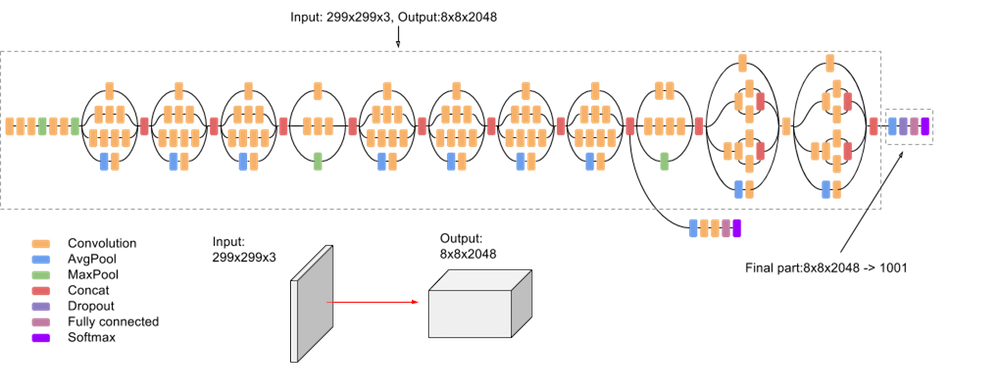
\includegraphics[scale=0.5]{images/ch4/inceptionv3.png}
	\caption{Overview of the Inception v3 network architecture. Source \href{https://cloud.google.com/tpu/docs/inception-v3-advanced}{Google's Advanced Guide to Inception v3 on Cloud TPU}}
	\label{fig:inceptionv3}
\end{figure}

This network receives an image represented by a 3D tensor with shape $(229, 229, 3)$, and generates an output consisting of 1001 logits, corresponding to the 1000 classification categories in the ImageNet dataset, plus an additional output to denote \textit{other} things not included in the labeled categories. However, we are interested in the last convolutional layer, just before entering the fully connected block. The output of a convolutional layer is a feature map organized as a grid of image patches and a number of features per image patch --the depth, or number of channels (see \cref{subsec:conv_layers}). As shown in \cref{fig:inceptionv3}, the output of the Inception-v3 network's last convolutional layer consists of $8 \times 8 \times 2048$ features, or in general, a 3D tensor of shape $(f_w, f_h, f_c)$, where $f_w$ and $f_h$ are the width and height of the feature map, respectively, and $f_c$ is the number of channels. However, instead of using this map as it is, it is squashed into a 2D tensor, with shape $(f_w \times f_h, f_c)$.

Finally, the squashed output of the last convolutional layer is fed into a \textbf{fully connected layer} with a ReLu activation function. This layer contains a certain number $D$ of units, which is an hyperparameter of the model. After forwarding the features map across this layer, we obtain as output a 2D tensor with shape $(L, D)$, where $L$ is the number of image patches, and $D$ is the number of features used to encode each patch (the number of units of the fully connected layer). Note that from an implementation viewpoint, due to the use of batch processing, we should consider another dimension in our data, the batch size. However, from a mathematical perspective, and for the sake of simplicity, we can ignore this additional dimension. 

All in all, hereafter, we will use the following notation to represent the output of the encoder. 
Let us call each set of features for a certain image patch as an \textit{annotation} vector, denoted by $a_i$. Then, the set of feature vectors can be defined as:

$$a = \{\text{a}_1,...,\text{a}_L \}, \text{a}_i \in \mathbb{R}^D$$

This approach uses the features of the convolutional layer instead of the the fully connected layer of the encoding CNN. This will allow the decoder to selectively focus on certain parts of an image by weighting a subset of all the feature vectors.

In our system, the number of features $L$ used to encode images is a configurable hyperparameter (\lstinline{config.num_features}), as is the name of the specific CNN used to extract image features (\lstinline{config.cnn}).

\section{Decoder}\label{sec:decoder}

The goal of the decoder is to generate a caption for the input image, that is, a  sentence that describes what can be seen in the image. We will use $y$ to denote the output of the decoder, which is a sequence of the outputs generated at each time step.

$$y = \{\text{y}_1,..., \text{y}_c\}, \text{y}_i \in \mathbb{R}^K$$

where $K$ is the size of the vocabulary (number of words), and $C$ is the length of the caption.
Each output $y_i$ is a vector with size $K$ that represents a probability distributions over the language vocabulary. That is, each element represents the probability of choosing one specific word. There are different ways to choose the final sentence from this sequence of probability distributions, as we will discuss later in this chapter.

The core element of the decoder is a single \textbf{recurrent layer} (named \textbf{RNN} in \cref{fig:overall-architecture}), which consists of a number of recurrent unit with hidden state, either GRU or LSTM units indistinctly. Both the type of recurrent unit and the number of units are hyperparameters of the model \footnote{For a description of how recurrent units work the reader is referred to \cref{subsec:rnn}, and more specifically, the section on recurrent units with hidden state (\cref{subsubsec:rnn_with_hidden_state}). There are also specific sections on GRU (\cref{subsec:gru}) and LSTM (\cref{subsec:lstm}) units}.

In addition to the recurrent layer, the encoder also comprises an embedding layer and two fully connected layers stacked on top of the recurrent layer. 

The \textbf{embedding layer} takes an input consisting of a word token, and transforms it into a dense vector embedding using an embedding matrix $E \in \mathbb{R}^{m \times K}$, where $m$ is the dimension of the embedding vector. During the caption generation process, the input to the embedding layer is the last token generated, so we denote the result of the embedding as $E\text{y}_{t-1}$.

The input to the recurrent layer at a given timestep $t$ will consist of both the result of the embedding layer $E\text{y}_{t-1}$, a context vector $\hat{z}_t$ coming from the attention mechanism, as well as the previous hidden state $\text{h}_{t-1}$. 

The context vector $\hat{z}_t$ is a dynamic representation of the relevant part of the image input at time $t$. Its computation is described in the next section.

The fully connected layers FC1 and FC2 constitute an MLP that is used to generate a sequence of words based on the output of the RNN. These two layers make a projection of the hidden state space into the output space. FC1 simple projects the RNN output into a tensor of shape $(C, n)$, where $C$ is the maximum sentence length, and $n$ is the number of RNN units. FC2 takes the output from FC1 and projects it into the final output space, that is, the language model. In particular, this final output is a sequence  $\{\text{y}_1,..., \text{y}_c\}$ of probability distributions of words in the vocabulary. That is, each element $y_i$ is a 1D tensor with shape $(K)$, made of values in [0,1] representing the probability of a different word from the language vocabulary. The are different methods to convert these probability distributions into a sentence, some which will be described later (\cref{sec:inference}).

\subsection{Attention}\label{subsec:attention}

The attention mechanism is responsible of deciding on which parts of the image to focus on at each timestep. In particular, we have designed an attention mechanism inspired by the model described in \textit{Show, Attend and Tell}, by \citet{Xu2015}, which is in turn based on the mechanism proposed by \citet{Bahdanau2015} as an addition to the \textit{seq2seq} model. More specifically, we replicate the  \textit{soft} attention mechanism proposed in the paper. This mechanism weights the features of each part of the image depending on a relevance score that is computed taking into account the current state of the decoder. This type of attention is called \textit{soft}, or \textit{global}, because it attends to the entire input space, unlike \textit{hard}/\textit{local} mechanisms, which attend to a specific location of the input space at any given moment, i.e. a patch of the image. Furthermore, this is a deterministic form of attention, as opposed to stochastic mechanisms, which use probability distributions to select the part of the input to focus at. Finally, this form attention can also be classified as self-attention, since the decoder attends to the encoder to generate its output, but it is also guided by its own internal state, as we will soon describe more formally.

The output of the attention mechanism is called the context vector $\hat{z}_t$ we have already introduced. Now let us see how this vector is computed.

We define a mechanism $\phi$ that computes $\hat{z}_t$ from the annotation vectors $\text{a}_i, i =1,...,L$ corresponding to the features extracted at different image locations. For each location $i$, the mechanism generates a positive weight $\alpha_i$ which is interpreted as the relative importance to give to location $i$ in blending the $\text{a}_i$'s together. The weight $\alpha_i$ of each annotation vector $\text{a}_i$ is computed by an \textit{attention model} $f_\text{att}$ for which we use a multilayer perceptron (not depicted in \cref{fig:overall-architecture}), conditioned on the previous hidden state $\text{h}_{t-1}$. To emphasize, note that the hidden state varies as the RNN advances in its output sequence: "where" the network looks next depends on the sequence of words that has already been generated (represented by the hidden state).

\begin{equation}\label{eq:att-scores}
 e_{ti} = f_\text{att}(\text{a}_i, \text{h}_{t-1})  
\end{equation}

The attention weights can be computed from the attention scores $e_{ti}$ by scaling to $[0,1]$ and normalizing (making weights sum to one).

\begin{equation}\label{eq:att-weights}
\alpha_{ti} = \frac{\exp{(e_{ti})}}{\sum_{k=1}^L \exp{(e_{tk})}}
\end{equation}

The attention weights represent the alignment between parts of the image and words in the caption that is being generated, as we will later illustrate with some pictures. Once the attention weights are computed, the context vector $\hat{z}_t$ can be computed by:

\begin{equation}\label{eq:att-context-1}
\hat{z}_t = \phi (\{\text{a}_i\},\{\alpha_i\})
\end{equation}

where $\phi$ is a function that returns a single context vector given the set of annotation vectors and their corresponding weights. There are different approaches to formulate this function depending on the attention model being used. On the one hand, learning a hard --stochastic-- attention model, requires sampling the attention locations $s_t$ each timestep. However, for a soft attention model we can take the expectation of the context vector $\hat{z}_t$ directly,

$$\mathbb{E}_{p(s_t|a)}[\hat{z}_t] = \sum_{i=1}^L \alpha_{ti}\text{a}_i,$$

and formulate a deterministic attention model by computing a weighted annotation vector

\begin{equation}\label{eq:att-context-2}
\phi(\{\text{a}_i\}, \{\alpha_i\}) = \sum_{i=1}^L \alpha_i\text{a}_i,
\end{equation}

as proposed by \citet{Bahdanau2015}. These weighted vectors $\alpha_i$ are used as a soft context that weights the different parts of the image with variable degrees of relevance, depending on the state of the decoder, ie. the sentence that has been generated so far. The whole model is smooth and differentiable under deterministic attention, so learning end-to-end is trivial by using standard back-propagation.

In particular, to compute the attention weights $\alpha$ we first compute the scores $e_{eti}$ using the additive scoring mechanism proposed by \citep{Bahdanau2015}. This mechanism can be implemented by a multilayer perceptron with a \textit{tanh} activation function applied over the addition of the annotation vector (the image features for different image locations), and the hidden state of the decoder's RNN.

More formally, the \textit{attention model} $f_\text{att}$ is formulated as:

\begin{equation}\label{eq:att-model}
f_\text{att} = v_a^{\top} \tanh(W_1 a_t + W_2 h_{t})
\end{equation}

where $W_1$, $W_2$, and $V_a$ are weights to be learned by backpropagation during the training phase. 

Finally, note that computing the attention weights $\alpha_i$ as defined in \cref{eq:att-weights} is equivalent to applying a \textit{softmax} function over the attention scores $e_{ti}$. Therefore, equations \cref{eq:att-scores} and \cref{eq:att-model} can be implemented by a combination of three fully connected layers and two activation functions, as depicted in \cref{fig:attention-architecture}.

\begin{figure}[hpt]
	\centering
	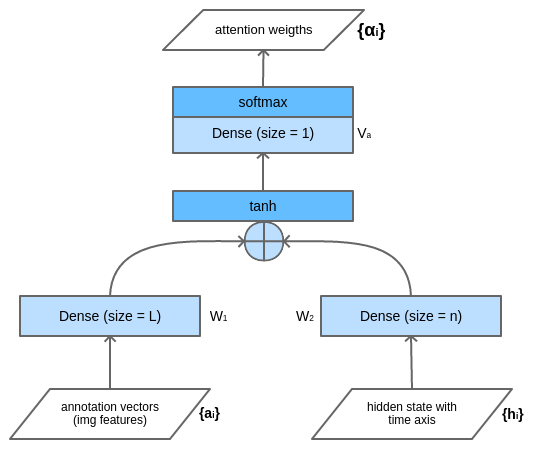
\includegraphics[scale=0.6]{images/ch4/attention-architecture.png}
	\caption{Detailed architecture of the additive soft attention mechanism}
	\label{fig:attention-architecture}
\end{figure}

In our model, the number of units, and thus the dimension of the hidden state, is a configurable hyperparameter (\lstinline{config.rnn_units}). In addition, the type of RNN unit to use is also specified as an hyperparameter (config.rnn) with two possible values: 'gru' or 'lstm'.

\section{Data pipelines}

This section describes the data preparation steps needed to train our model over a benchmark dataset such as MS COCO. Fitting a model over a big dataset will require processing large amounts of data, and thus may highly benefit from as much parallelization as possible. To that aim, we will organize our data to support parallel pipeline processing by leveraging data parallelization structures, such as the \lstinline{Dataset} class available in \lstinline{Tensorflow}.

A general overview of the data pipeline is provided in \cref{fig:data-pipelines}. It all begins with a raw dataset, as the COCO dataset, which consists of a number of images and associated captions in some dataset-specific format. Then, we perform separate preprocessing tasks for the images and for the captions. In order to accelerate training and evaluation tasks, image features are computed once and cached to disk. Once image features have been extracted and cached, and the captions have been converted into sequences ready to be set into the RNN, images and their associated sequences are combined into parallel-efficient data structures supporting buffering and batching. If the data is being used for training, then it is also randomly shuffled before generating batches.

\begin{figure}[hpt]
	\centering
	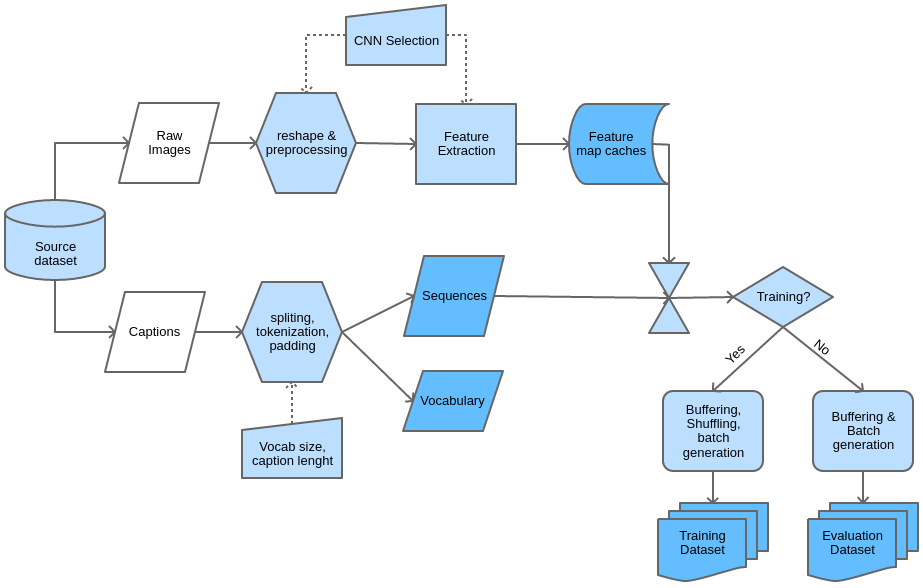
\includegraphics[scale=0.5]{images/ch4/data-pipelines.png}
	\caption{Overview of the data preparation pipeline}
	\label{fig:data-pipelines}
\end{figure}

The section is organized as follows, first we describe the pre-processing steps required to prepare images for the pipeline, then we describe the steps required to prepare the captions, and finally we describe the way images and captions are collated together into parallel efficient structures before being fed to the training or evaluation processes.

\subsection{Image pre-processing}

Images have to be encoded by a CNN to extract the visual features needed by the decoder. In order to be fed into the CNN, images have to be preprocessed first, which includes resizing them to the shape required by the particular CNN being used, as well as applying tweaks that are specific of each particular CNN. Some models use images with values ranging from 0 to 1, others from -1 to +1, yet others use the \textit{Caffe}\footnote{\textit{Caffe} is an open source deep learning framework, originally developed at University of California, Berkeley. More info can be found at the \href{http://caffe.berkeleyvision.org/}{official website}.} style, that is not normalized, but is centered. 

To support using different CNNs for the encoder, we have developed a generic method that can preprocess images for different models, including the following:

% \begin{table}[]
% \caption{Summary of ConvNets available for the encoder}
% \label{tab:my-table}
% \begin{tabular}{llll}
% CNN Model &  Image size & Features size & Reference paper & More info\\
% \hline
% VGG16 &  $224 \times 224$ & \citep{Simonyan2015} & \cref{cnn:vgg}\\
% Inception-V3 & $299 \times 299$ &\citep{Szegedy2016}& \cref{cnn:googlenet}\\
% ResNet50 & $224 \times 224$ &\citep{He2016resnet}& \cref{cnn:resnet}\\
% Xception & $299 \times 299$ &\citep{Chollet2017}& \\
% NASNetLarge & $331 \times 331$ &\citep{Zoph2018}& \\
% \end{tabular}
% \end{table}

\begin{table}[hpt]
\caption{Summary of  popular ConvNets pretrained on the ImageNet dataset}
\label{tab:popular-convnets}
\begin{tabular}{lllllll}
Model & Image size & Weights size & Top-1 acc. & Top-5 acc. & Params & Depth \\
\hline
Xception & 299 x 299 & 88 MB & 0.790 & 0.945 & 22,910,480 & 126 \\
VGG16 & 224 x 224 & 528 MB & 0.715 & 0.901 & 138,357,544 & 23 \\
VGG19 & 224 x 224 & 549 MB & 0.727 & 0.910 & 143,667,240 & 26 \\
ResNet50 & 224 x 224 & 99 MB & 0.759 & 0.929 & 25,636,712 & 168 \\
InceptionV3 & 299 x 299 & 92 MB & 0.788 & 0.944 & 23,851,784 & 159 \\
InceptResNetV2 & 299 x 299 & 215 MB & 0.804 & 0.953 & 55,873,736 & 572 \\
MobileNet & 224 x 224 & 17 MB & 0.665 & 0.871 & 4,253,864 & 88 
\end{tabular}
\end{table}

Images can be encoded into feature maps beforehand, that is, prior to using them for training or inference purposes. That means we only need to generate the image feature maps once and save them to disk. To do that aim, in addition to having commands for the training and evaluation steps, we have also included a command called \lstinline{prepare} which simply generates and saves to disk image features for a certain CNN. 

It is important to remark that for encoding images we are using the features obtained by the last convolutional layer of the network, excluding the fully connected parts that use to lie at the top, since these networks are pretrained for a classification task\footnote{Typically these models have the weights of the networks that participated in some edition of the ImageNet Large Scale Visual Recognition Competition (ILSVRC)}.
The size of the feature maps generated by the encoding process also differs for different ConvNets. These maps are encoded as grids made of image patches with a certain width $W$, height $H$, and depth $D$. Note that the depth is simply the number of features per patch, and is equal to the number of channels of the last convolution layer. For example, the InceptionV3 model produces feature maps with shape $(8 \times 8 \times 2048)$. However, in the end all the image features will be passed through a fully connected layer that will squash them into 2D tensor with shape $(L,D)$, as described in section \cref{sec:encoder}. 

The specific pretrained CNN to use in the encoder constitutes an hyperparameter of the model (\lstinline{config.cnn}) which may adopt the following values: 'vgg16', 'resnet50', 'inception', 'xception', and 'nasnet\_large' (although we were unable to use the latest due to lack of memory).

\subsection{Text pre-processing}

Captions are short sentences in natural language. The ultimate goal of the image captioning problem is to generate captions for new images not included in the training dataset. Therefore, the task of generating a caption can be seen as a task of predicting a sequence of symbols, which implies learning some model of the language. For building such models, we need to turn text into a format that we can optimize over, i.e. we need to map sentences of the language into numerical vectors. These vectors provide a numerical representation of the symbols in the language. First of all, we must decide on the level of granularity used to represent the symbols of the language. One strategy is to treat each word as a unique entity, e.g. \citep{Salton1975}. At the other extreme lies the strategy to predict one character at a time, as suggested e.g. by \citet{Ling2015} \footnote{Actually, another alternative between both strategies is byte-pair encoding, as described by \citet{Sennrich2016} for the purpose of neural machine translation. It decomposes text into syllable-like fragments that occur frequently. This allows for models that are able to generate words like heteroscedastic or pentagram based on previously viewed words, e.g. heterogeneous, homoscedastic, diagram, and pentagon}. 

Going into details about language models is beyond the scope of this section. Here it suffice to say that we need an strategy to convert textual captions into sequence of tokens. A token is a data point the model will train and predict. For seq2seq tasks like translation and image captioning the most common approach is to use words as tokens, and that is the approach we adopt here.

\subsubsection{Tokenization and language modelling}\label{subsec:tokenization}

To begin with, we need to split captions into tokens, that is, words. As part of this process we will also remove non alphanumeric characters and punctuation marks. 

Then, we need to map tokens into numerical indices. We often call it a \textit{vocabulary}. Its input is a list of tokens, called a corpus. Then it counts the frequency of each token in this corpus, and assigns a numerical index to each token according to its frequency, from most frequent to more rare tokens. The size of the vocabulary is limited, so that rare tokens are removed to reduce the complexity. In order to mark the beginning and end of a sentence, two special tokens are added to the vocabulary: a token named "<start>" (also  named "<sos>" or "<bos>") to mark the beginning of sentence, and "<end>" (or "<end>") for the ending of a sentence. Furthermore, another token named "<unk>" is used to represent words that are not included in the vocabulary. Finally, since we may be representing sentences of different length, we also need an special token named "<pad>" for padding shorter sentences. It is common practice to use 0 as the index of the "<pad>" token, so that it is ignored (it has no activation effects).  

In our system, the corpus is made of all the captions included in the training dataset. We have included configuration options to limit the number of words in the vocabulary. For example, for the COCO dataset, the complete corpus consists of almost 30,000 words, but we have limited the vocabulary size to 10,000 words, which seems to be a reasonable size. This vocabulary only has to be built once, since it can be saved and loaded from disk. Needless to say that the vocabulary must be rebuild whenever a new corpus is used or the existing corpus changes. The size of the vocabulary is a configurable hyperparameter of our model (\lstinline{config.vocabulary_size}).

\paragraph{One-Hot encoding}
One-hot encoding vectors provide an easy way to express words as vectors in order to process them in a deep network. In a nutshell, we map each word to a different unit vector: assume that the number of different words in the dictionary is $K$ and each word has a one-to-one correspondence with a single value in the index of successive integers from 0 to $K-1$. If the index of a word is the integer $i$, then we create a vector $\mathbf{e}_i$ of all 0s with a length of $K$ and set the element at position $i$ to $1$. This vector is the \textit{one-hot} vector representation of the original word. 

\paragraph{Word embeddings}\label{subsubsubsec:}

One-Hot vectors provide an sparse vector representation of words. \textit{Word embedding}, however, refer to a technique that uses dense, vectors of real numbers to represent words. Such a vector can be thought of as the feature vector of a word.  

Although one-hot word vectors are easy to construct, they are usually not a good choice. One of the major reasons is that the one-hot word vectors cannot accurately express the similarity between different words, such as the cosine similarity that we commonly use. For the vectors $\mathbf{x}, \mathbf{y} \in \mathbb{R}^d$, their cosine similarities are the cosines of the angles between them:

$$\frac{\mathbf{x}^\top \mathbf{y}}{\|\mathbf{x}\| \|\mathbf{y}\|} \in [-1, 1].$$

Since the cosine similarity between the one-hot vectors of any two different words is 0, it is difficult to use the one-hot vector to accurately represent the similarity between multiple different words.

There are various approaches to learn the word embeddings space, being the \textit{skip-gram}\citep{Mikolov2013} and the \textit{bag-of-words} (BoW) \footnote{The BoW model is a simplifying representation used in natural language processing and information retrieval (IR). In this model, a text is represented as the bag (multiset) of its words, disregarding grammar and even word order but keeping multiplicity. This model dates from Zellig Harris's 1954 article on Distributional Structure} are two of the most popular. 

Although there exist open source tools (eg. Word2Vec) and pretrained language models (Glove) available, for this project we decided to take another approach: learning the embedding matrix as an integral part of the complete, end-to-end learning process. This can be a slower approach, but tailors the language model to the task at hand and the specific dataset. 

From a practical viewpoint, learning a tailored model can be achieved simply by adding an \textit{embedding} layer as the first layer of the decoder, as described above (section \cref{sec:decoder}). That way, we will not need to embed the words beforehand, as a previous step. Instead, the embedding matrix will be learned just as any other layer of the model, and it will suffice with providing a one-hot encoding representation of captions to train the model.

Such an embedding layer has tw hyperparameters that are added to our model as configurable options: the size of the vector space in which words will be embedded (\lstinline{config.embedding_dim}), and the size of the vocabulary (\lstinline{config.vocabulary_size})

\subsection{Dataset generation}

We have already described the image preprocessing steps and the text preprocessing that has to be carried out to prepare our data prior to using it. However, in order to efficiently use this data as input to the full pipeline of our end-to-end model, we need to organize it into special data structures supporting batching, shuffling, prefetching (buffering), and parallelism. Fortunately, Tensorflow a data structure supporting all those features, by the name of \lstinline{Dataset}. This structure allows to link together different data sources, as long as the data can be converted to tensors, which includes all primitive data types. That means we can build an instance of \lstinline{Dataset} that collates together the feature maps obtained from a set of images, and the one-hot tokenized representations of the captions associated to those images. Therefore, we could prefetch, shuffle and organize that data in batches.

In our system, we have added the batch size as an hyperparameter that can be customized (\lstinline{config.batch_size}). 

We have created methods to create two different Dataset instances, one for the training portion of the image-caption dataset, and another one its the evaluation portion.

\section{Training the model}\label{sec:training}

Training is the process of fitting the model to a particular dataset. In many tasks, including image captioning, training is supervised, that is, dataset instances are labelled with the solutions. In this cases, the model is fitted to the data by modifying its parameters (eg. the weights of a neural network) so that a particular loss function is minimized.

In the image captioning problem, the data examples are the images, and the labels are the captions, expressed in natural language. Usually these captions are provided by humans that were asked to describe the images\footnote{This can be done in large quantities thanks to crowdsourcing marketplaces like the \href{https://www.mturk.com/}{ Amazon Mechanical Turk (MTurk)}.}. In this particular case, the loss function is computed by comparing word by word the sentence generated by the RNN against the provided caption. However, due to the sequential nature of the output this is not as simple as computing the loss with non sequential outputs, like typically happens when solving a classification task. In particular, we will use a specific technique used for learning sequential models which is called \textbf{Teacher Forcing}, which is explained below.

\subsection{Loss function}\label{subsec:loss_function}

In order to use supervised training, we need to minimize a loss function. In the image captioning problem, the error will be related with the generation of the caption: the actual caption constitutes the ground truth, while the caption generated by the model will be the prediction. However, a sequence is not generated in a single step, instead it is computed word by word, and the loss will be computed word by word. Let us see how the training unfolds sequentially in order to understand how to compute a loss function.

On the one hand, the image associated to the example caption is processed by the encoder ConvNet and results in a 2D tensor of features, which are then weighted by the attention mechanism, and conveniently reshaped before being fed into the decoder RNN as. The resulting tensor corresponds to the \textit{context} explained above (\cref{subsec:attention}): $\hat{z}_t$

On the other hand, the caption is converted into a sequence of embedding vectors, once per each word ($Ex_t$).  The word embeddings have to be concatenated with the context vectors to produce the final input to the RNN, but this process does not happen as a single step. Instead, the word embeddings have to be processed one by one, and for each embedding $Ex_t$  a new context vector will computed by the attention mechanism and concatenated to make the input at timestep $t$:

$$[\hat{z}_t;Ex_t]$$

Given that input and the previous hidden state $t_{t-1}$, the RNN will generate a new output $y_t$. The output is a vector of \textit{logits} with dimension equals to the number of words in vocabulary, $K$. That is, each element of the output vector is the probability of a word in the vocabulary. Such output can be interpreted as the prediction of a particular word, so that it can be compared against the ground truth to compute a loss value, where the grount truth refers to the actual word in the $t^{th}$ position of the caption. This can be seen as a multitask classification task, with as many classes as words in the vocabulary. Furthermore, since the ground truth is represented using one-hot encoding, then we should use  a \lstinline{SparseCategoricalCrossentropy} loss function to compute the loss between the predicted word and the actual word.

The losses for every word in the sentence will be computed separately and summed together to obtain a single loss value. Finally, the accumulated loss shall be divided by the length of the caption to obtain a loss value that is independent of the length of the caption.

Besides, when computing the loss value, padding tokens should be avoided, which is done by means of masking. 

\begin{lstlisting}
def compute_loss(labels, predictions, loss_function):
    mask = tf.math.logical_not(tf.math.equal(labels, 0))
    loss_ = loss_function(labels, predictions)

    mask = tf.cast(mask, dtype=loss_.dtype)
    loss_ *= mask

    return tf.reduce_mean(loss_)
\end{lstlisting}


\subsection{Teacher forcing}\label{subsec:teacher_forcing}

There are sequence prediction models that use the output from the last time step $y_{t-1}$ as input for the model at the current time step $X_t$. This type of model is common in language models that output one word at a time and use the output word as input for generating the next word in the sequence.
For example, this type of language model is used in an Encoder-Decoder recurrent neural network architecture for sequence-to-sequence generation problems such as: machine translation, text summarization, question answering, and image captioning.

\textit{Teacher forcing} is a strategy for training recurrent neural networks that uses model output from a prior time step as an input. This method was originally proposed as an alternative technique to backpropagation through time for training a recurrent neural network \citep{Williams1989}.

Teacher forcing works by using the expected output from the training dataset at the current time step $t$ as input in the next time step $t+1$, rather than the output generated by the network, as is the case when the network is predicting a new sequence (as is the case during the validation stage). Let us explain teacher forcing with a concrete example.

Consider an image of a tennis player with the following caption:

\begin{verbatim}
<start> a man standing on a tennis court holding a tennis racquet <end>    
\end{verbatim}

\cref{fig:teacher-forcing} depicts the inputs at each time step for the example above. We are not showing the outputs here because it is not relevant. The loss function will be computing between pairs (input, output), aggregated and divided by the length of the caption.

\begin{figure}[hpt]
	\centering
	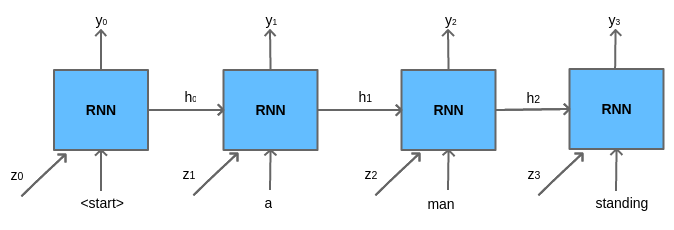
\includegraphics[scale=0.5]{images/ch4/teacher-forcing.png}
	\caption{Teacher forcing for image captioning training. The expected word is used as input of the network at each timestep}
	\label{fig:teacher-forcing}
\end{figure}

Teacher forcing is a fast and effective way to train a recurrent neural network that uses output from prior time steps as input to the model. Nevertheless, this approach can also result in models with poor prediction performance as the RNN’s conditioning context (the sequence of previously generated samples) diverge from sequences seen during training\citep{Lamb2016}. This is common in most applications of this type of model as the outputs are probabilistic in nature. This type of application of the model is often called open loop.

\section{Inference and validation}\label{sec:inference}

After the model is trained, it can be used to generate new sequences. To do that, we should simply fed a "<start>" token to the RNN start the process, and the generated word in the output sequence will then be used as input on the subsequent time step (along with the context vector coming from the attention mechanism).

\begin{figure}[hpt]
	\centering
	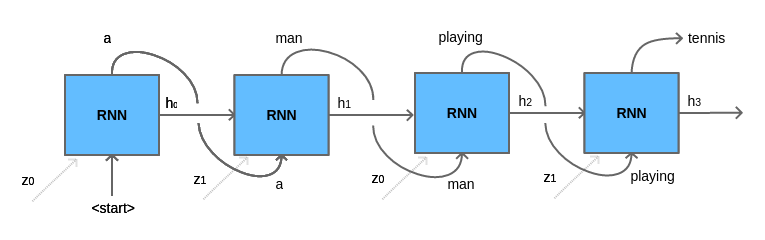
\includegraphics[scale=0.5]{images/ch4/inference.png}
	\caption{Word-by-word caption generation}
	\label{fig:teacher-forcing}
\end{figure}

The generation process will continue until the "<end>" token is reached, or a maximum sequence length is reached.

Various approaches exist to predict the next token. For example, in greedy search, the token with the highest score at each time step is chosen and used to predict the next token. However, there are more sophisticated approaches, introduce below. 

For ease of discussion, we assume that the output of the decoder is a sequence of text. Let the size of output text dictionary $\mathcal{Y}$ (contains special symbol "<end>") be $\left|\mathcal{Y}\right|$, and the maximum length of the output sequence be $T'$. There are a total $\mathcal{O}(\left|\mathcal{Y}\right|^{T'})$ types of possible output sequences. All the subsequences after the special symbol "<end>" in these output sequences will be discarded.

\subsection{Greedy Search}\label{subsec:greedy-search}

First, we will take a look at a simple solution: greedy search. For any time step $t'$ of the output sequence, we are going to search for the word with the highest conditional probability from $|\mathcal{Y}|$ numbers of words, with

$$y_{t'} = \operatorname*{argmax}_{y \in \mathcal{Y}} \mathbb{P}(y \mid y_1, \ldots, y_{t'-1}, \boldsymbol{c})$$

as the output.  Once the "<end>" symbol is detected, or the output sequence has reached its maximum length $T'$, the output is completed.

As we mentioned in out discussion of the decoder, the conditional probability of generating an output sequence based on the input sequence is $\prod_{t'=1}^{T'} \mathbb{P}(y_{t'} \mid y_1, \ldots, y_{t'-1}, \boldsymbol{c})$. We will take the output sequence with the highest conditional probability as the optimal sequence. The main problem with greedy search is that there is no guarantee that the optimal sequence will be obtained.

Take a look at the example in \cref{fig:s2s_prob1}. We assume that there are four words "A", "B", "C", and "<end>" in the output dictionary.  The four numbers under each time step represent the conditional probabilities of generating "A", "B", "C", and "<end>" at that time step.  At each time step, greedy search selects the word with the highest conditional probability. Therefore, the output sequence "A", "B", "C", "<end>" will be generated in \cref{fig:s2s_prob1}. The conditional probability of this output sequence is $0.5\times0.4\times0.4\times0.6 = 0.048$.


\begin{figure}[hpt]
	\centering
	\includesvg{images/ch4/s2s_prob1.svg}
	\caption{The four numbers under each time step represent the conditional probabilities of generating "A", "B", "C", and "<end>" at that time step. At each time step, greedy search selects the word with the highest conditional probability.}
	\label{fig:s2s_prob1}
\end{figure}

% TODO many error in references to figures in the next paragraph

Now, we will look at another example shown in \cref{fig:s2s_prob2}. Unlike in \cref{fig:s2s_prob1}, \cref{fig:s2s_prob2} selects the word "C" for it has the second highest conditional probability at time step 2. Since the output subsequences of time steps 1 and 2, on which time step 3 is based, are changed from "A" and "B" in \cref{fig:s2s_prob1} to "A" and "C" in \cref{fig:s2s_prob2}, the conditional probability of each word generated at time step 3 has also changed in \cref{fig:s2s_prob2}. We choose the word "B", which has the highest conditional probability. Now, the output subsequences of time step 4 based on the first three time steps are "A", "C", and "B", which are different from "A", "B", and "C" in \cref{fig:s2s_prob1}. Therefore, the conditional probability of generating each word in time step 4 in \cref{fig:s2s_prob2} is also different from that in \cref{fig:s2s_prob1}. We find that the conditional probability of the output sequence "A", "C", "B", "<end>" at the current time step is $0.5\times0.3 \times0.6\times0.6=0.054$, which is higher than the conditional probability of the output sequence obtained by greedy search. Therefore, the output sequence "A", "B", "C", "<end>" obtained by the greedy search is not an optimal sequence.

\begin{figure}[hpt]
	\centering
	\includesvg{images/ch4/s2s_prob2.svg}
	\caption{The four numbers under each time step represent the conditional probabilities of generating "A", "B", "C", and "<end>" at that time step.  At time step 2, the word "C", which has the second highest conditional probability, is selected.}
	\label{fig:s2s_prob2}
\end{figure}

\subsection{Exhaustive Search}\label{subsec:exhaustive-search}

If the goal is to obtain the optimal sequence, we may consider using exhaustive search: an exhaustive examination of all possible output sequences, which outputs the sequence with the highest conditional probability.

Although we can use an exhaustive search to obtain the optimal sequence, its computational overhead $\mathcal{O}(\left|\mathcal{Y}\right|^{T'})$ is likely to be excessively high. For example, when $|\mathcal{Y}|=10000$ and $T'=10$, we will need to evaluate $10000^{10} = 10^{40}$ sequences. This is next to impossible to complete. The computational overhead of greedy search is $\mathcal{O}(\left|\mathcal{Y}\right|T')$, which is usually significantly less than the computational overhead of an exhaustive search. For example, when $|\mathcal{Y}|=10000$ and $T'=10$, we only need to evaluate $10000\times10=1\times10^5$ sequences.

\subsection{Beam Search}\label{subsec:beam-search}

Beam search is an improved algorithm based on greedy search. It has a hyper-parameter named beam size. We set it to $k$. At time step 1, we select $k$ words with the highest conditional probability to be the first words of the $k$ candidate output sequences. For each subsequent time step, we are going to select the $k$ output sequences with the highest conditional probability from the total of $k\left|\mathcal{Y}\right|$ possible output sequences based on the $k$ candidate output sequences from the previous time step. These will be the candidate output sequence for that time step. Finally, we will filter out the sequences containing the special symbol "<end>" from the candidate output sequences of each time step and discard all the subsequences after it to obtain a set of final candidate output sequences.

\begin{figure}[hpt]
	\centering
	\includesvg{images/ch4/beam_search.svg}
	\caption{The beam search process. The beam size is 2 and the maximum length of the output sequence is 3. The candidate output sequences are $A$, $C$, $AB$, $CE$, $ABD$, and $CED$. }
	\label{fig:beam_search}
\end{figure}

\cref{fig:beam_search} demonstrates the process of beam search with an example. Suppose that the vocabulary of the output sequence only contains five elements: $\mathcal{Y} = \{A, B, C, D, E\}$ where one of them is a special symbol “<end>”. Set beam size to 2, the maximum length of the output sequence to 3. At time step 1 of the output sequence, suppose the words with the highest conditional probability $\mathbb{P}(y_1 \mid \boldsymbol{c})$ are $A$ and $C$. At time step 2, we compute $\mathbb{P}(A, y_2 \mid \boldsymbol{c}) = \mathbb{P}(A \mid \boldsymbol{c})\mathbb{P}(y_2 \mid A, \boldsymbol{c})$ and $\mathbb{P}(C, y_2 \mid \boldsymbol{c}) = \mathbb{P}(C \mid \boldsymbol{c})\mathbb{P}(y_2 \mid C, \boldsymbol{c})$ for all $y_2 \in \mathcal{Y}$, and pick the largest two among these 10 values: say $\mathbb{P}(A, B \mid \boldsymbol{c})$ and $\mathbb{P}(C, E \mid \boldsymbol{c})$. Then at time step 3, we compute $\mathbb{P}(A, B, y_3 \mid \boldsymbol{c}) = \mathbb{P}(A, B \mid \boldsymbol{c})\mathbb{P}(y_3 \mid A, B, \boldsymbol{c})$ and $\mathbb{P}(C, E, y_3 \mid \boldsymbol{c}) = \mathbb{P}(C, E \mid \boldsymbol{c})\mathbb{P}(y_3 \mid C, E, \boldsymbol{c})$ for all $y_3 \in \mathcal{Y}$, and pick the largest two among these 10 values: say $\mathbb{P}(A, B, D \mid \boldsymbol{c})$ and $\mathbb{P}(C, E, D \mid  \boldsymbol{c})$. As a result, we obtain 6 candidates output sequences: (1) $A$; (2)$C$; (3) $A$, $B$; (4)$C$, $E$; (5)$A$, $B$, $D$; and (6)$C$, $E$, $D$. In the end, we will get the set of final candidate output sequences based on these 6 sequences.

In the set of final candidate output sequences, we will take the sequence with the highest score as the output sequence from those below:

$$ \frac{1}{L^\alpha} \log \mathbb{P}(y_1, \ldots, y_{L}) = \frac{1}{L^\alpha} \sum_{t'=1}^L \log \mathbb{P}(y_{t'} \mid y_1, \ldots, y_{t'-1}, \boldsymbol{c}),$$

Here, $L$ is the length of the final candidate sequence and the selection for $\alpha$ is generally 0.75. The $L^\alpha$ on the denominator is a penalty on the logarithmic addition scores for the longer sequences above. The computational overhead $\mathcal{O}(k\left|\mathcal{Y}\right|T')$ of the beam search can be obtained through analysis. The result is a computational overhead between those of greedy search and exhaustive search. In addition, greedy search can be treated as a beam search with a beam size of 1. Beam search strikes a balance between computational overhead and search quality using a flexible beam size of $k$.

Note: In the developed system, we have implemented both greedy search and beam search, however, results with beamsearch hasn't been satisfactory. 

% The visualization of the attention weights clearly demonstrates which regions of the image the model pays attention to so as to output a certain word.
